\documentclass[tikz,border=2mm]{standalone}
\usepackage{amsmath}
\usetikzlibrary{positioning}

\newcommand{\myfontsize}{\fontsize{8pt}{12pt}\selectfont}

\begin{document}
	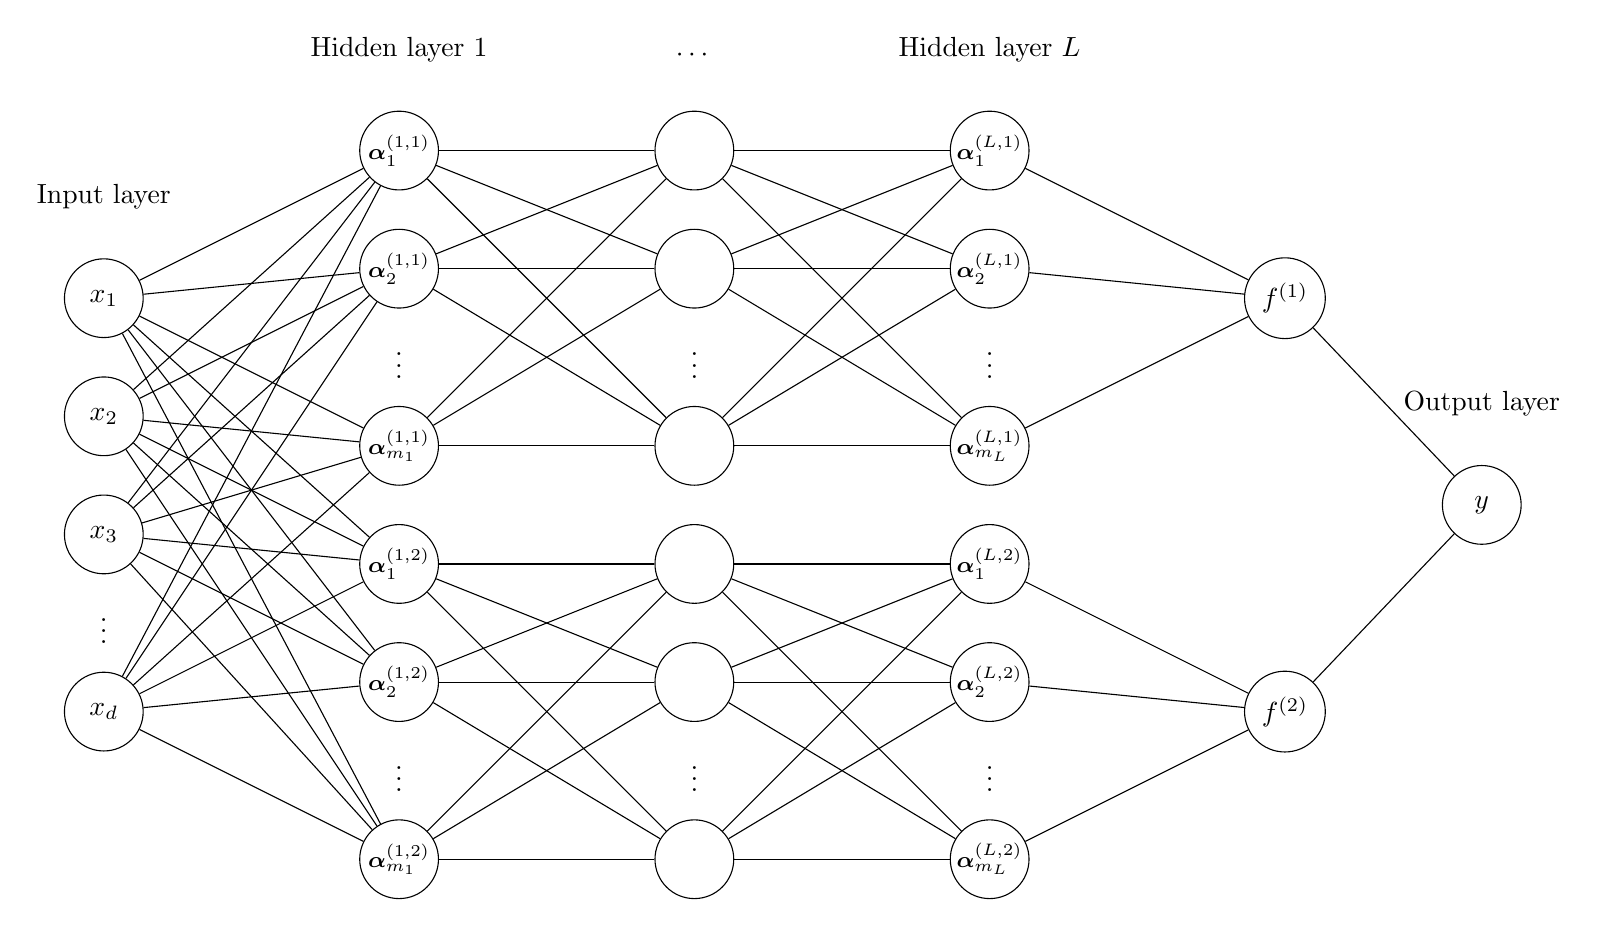
\begin{tikzpicture}[x=2.5cm, y=1.5cm, >=stealth]
\centering
		% input layer nodes
		\foreach \i in {1, ..., 3} {
			\node[circle, draw=black, fill=white, minimum size=1cm] (x\i) at (0, -\i+2.75) {$x_{\i}$};}
		\node at (0, -1) {$\vdots$};
		\node[circle, draw=black, fill=white, minimum size=1cm] (x4) at (0, -1.75) {$x_d$};

		
		% hidden layer 1 nodes
		\foreach \i in {1, ..., 2} {
			\node[circle, draw=black, fill=white, minimum size=1cm] (a11\i) at (1.5, -\i+4) {};
			\node at (1.5, -\i+4) [font=\myfontsize] {$\boldsymbol{\alpha}^{(1,1)}_{\i}$};}
     	\node at (1.5, 1.25) {$\vdots$};
		\node[circle, draw=black, fill=white, minimum size=1cm] (a113) at (1.5, 0.5) {};
	    \node at (1.5, 0.5) [font=\myfontsize] {$\boldsymbol{\alpha}^{(1,1)}_{m_1}$};
	
	    \foreach \i in {1, ..., 2} {
		    \node[circle, draw=black, fill=white, minimum size=1cm] (a12\i) at (1.5, -\i+3.5-3){};
		    \node at (1.5, -\i+3.5-3) [font=\myfontsize] {$\boldsymbol{\alpha}^{(1,2)}_{\i}$};} 
         \node[circle, draw=black, fill=white, minimum size=1cm] (a123) at (1.5, -3){};
         \node at (1.5, -2.25) {$\vdots$};
         \node at (1.5, -3) [font=\myfontsize] {$\boldsymbol{\alpha}^{(1,2)}_{m_1}$};
		
		
		% other hidden layers
		\foreach \i in {1, ..., 2} {
			\node[circle, draw=black, fill=white, minimum size=1cm] (a31\i) at (3, -\i+4) {};
			%\node at (4.5, -\i+4) [font=\myfontsize] {$\boldsymbol{\alpha}^{(i,1)}_{\i}$};
		}
		\node at (3, 1.25) {$\vdots$};
		\node[circle, draw=black, fill=white, minimum size=1cm] (a313) at (3, 0.5) {};
		%\node at (4.5, 0.5) [font=\myfontsize] {$\boldsymbol{\alpha}^{(3,1)}_{m_i}$};
		
		\foreach \i in {1, ..., 2} {
			\node[circle, draw=black, fill=white, minimum size=1cm] (a32\i) at (3, -\i+3.5-3){};
			%\node at (4.5, -\i+3.5-3) [font=\myfontsize] {$\boldsymbol{\alpha}^{(i,2)}_{\i}$};
		} 
		\node[circle, draw=black, fill=white, minimum size=1cm] (a323) at (3, -3){};
		\node at (3, -2.25) {$\vdots$};
		%\node at (4.5, -3) [font=\myfontsize] {$\boldsymbol{\alpha}^{(i,2)}_{m_i}$};
	
		% hidden layer L nodes
	    \foreach \i in {1, ..., 2} {
	    	\node[circle, draw=black, fill=white, minimum size=1cm] (aL1\i) at (4.5, -\i+4) {};
	    	\node at (4.5, -\i+4) [font=\myfontsize] {$\boldsymbol{\alpha}^{(L,1)}_{\i}$};}
	    \node at (4.5, 1.25) {$\vdots$};
	    \node[circle, draw=black, fill=white, minimum size=1cm] (aL13) at (4.5, 0.5) {};
	    \node at (4.5, 0.5) [font=\myfontsize] {$\boldsymbol{\alpha}^{(L,1)}_{m_L}$};
	    
	    \foreach \i in {1, ..., 2} {
	    	\node[circle, draw=black, fill=white, minimum size=1cm] (aL2\i) at (4.5, -\i+3.5-3){};
	    	\node at (4.5, -\i+3.5-3) [font=\myfontsize] {$\boldsymbol{\alpha}^{(L,2)}_{\i}$};} 
	    \node[circle, draw=black, fill=white, minimum size=1cm] (aL23) at (4.5, -3){};
	    \node at (4.5, -2.25) {$\vdots$};
	    \node at (4.5, -3) [font=\myfontsize] {$\boldsymbol{\alpha}^{(L,2)}_{m_L}$};
	
	    
		
		% hidden layer 5 nodes
		\node[circle, draw=black, fill=white, minimum size=1cm] (f1) at (6, 1.75){$f^{(1)}$};
		\node[circle, draw=black, fill=white, minimum size=1cm] (f2) at (6, -1.75){$f^{(2)}$};
		
		% output layer node
		\node[circle, draw=black, fill=white, minimum size=1cm] (o) at (7, 0) {$y$};
		
		% connections
		\foreach \i in {1, ..., 4} {
			\foreach \j in {1, ..., 3} {
				\draw (x\i) -- (a11\j);
				\draw (x\i) -- (a12\j);
			}
		}
		
	
	   	% new connection between hidden layer 1, 2 and 3
	    \foreach \i in {1,2,3} {
	   	    \foreach \j in {1,2,3} {
	   		    \draw (a11\i) -- (a31\j);
	   		    \draw (a12\i) -- (a32\j);
	   		    \draw (a31\i) -- (aL1\j);
	   		    \draw (a32\i) -- (aL2\j);
	   	    }
	   }
  
	   
		
		% connections between hidden layer 3 and 4
		\foreach \j in {1, ..., 3}{
	           \draw (aL1\j) -- (f1);\draw (aL2\j) -- (f2);}
           
        \draw (f1) -- (o);
        \draw (f2) -- (o);

% labels for layers
\node[above=0.5cm of a111] {Hidden layer 1};
\node[above=0.5cm of a311] {$\cdots$};
\node[above=0.5cm of aL11] {Hidden layer $L$};
%\node[above=0.5cm of f1] {Hidden layer $L+1$};
\node[above=0.5cm of x1] {Input layer};
\node[above=0.5cm of o] {Output layer};
\end{tikzpicture}
\end{document}